\chapter{Binary Search Complete Implementation}
\label{binappendix}
The best way to implement the tree data structure is to create a class for the nodes (\textbf{Node}) and a class for the binary tree (\textbf{BinaryTree}). As all the nodes of a binary trees has at most two children, in the class \textbf{Node} is enough to have three attributes: the value of the node, the left, and the right child, in turn of \textbf{Node} type as well. This way of implement tree is very similar to the one used for the linked list (\ref{linkedlist}).

\begin{lstlisting}[firstnumber=1, caption={Class definition for a node and a tree.}]
class Node():

	def __int__(self, value):
		self.value = value
		self.left = None
		self.right = None

class BinaryTree():

	def __init__(self, root):
		self.root = Node(root)
\end{lstlisting}

In this appendix there is a detailed implementation, both recursive and iterative, of all possible ways to perform a tree traversal in the case of depth-first search: pre-order traversal \ref{preorderappendix}, in-order traversal \ref{inorderappendix}, and post-order traversal \ref{postorderappendix}. The convention followed here is to look up first at the left child always, and later look up the right one. The opposite approach is equivalent.

\section{Pre-order Traversal}
\label{preorderappendix}

\begin{lstlisting}[firstnumber=1, caption={Recursive and iterative implementation of pre-order traversal.}]
class BinaryTree():
	...

	def print_tree(self):
		return self.preorder_print(tree.root, "")[:-1]

	def preorder_search_recursive(self, start, find_val):
		if start:
			if start.value == find_val:
				return True
			else:
				return preorder_search_recursive(start.left, find_val) or
					   preorder_search_recursive(start.right, find_val)

	def preorder_search_iterative(self, start, find_val):
		if start == None:
			return None
		stack = []
		stack.push(start)
		while not stack: # Keep cycle until the stack is empty
			node = stack.pop()
			if node == find_val:
				return True
			# Right child is pushed first so that the left one is processed first
			if node.right:
				stack.push(node.right)
			if node.left:
				stack.push(node.right)

	def preorder_print(self, start, traversal):
		if start:
			traversal += (str(start.value) + "-")
			traversal = self.preorder_print(start.left, traversal)
			traversal = self.preorder_print(start.right,traversal)
		return traversal
\end{lstlisting}

\begin{figure}[H]
	\begin{center}
		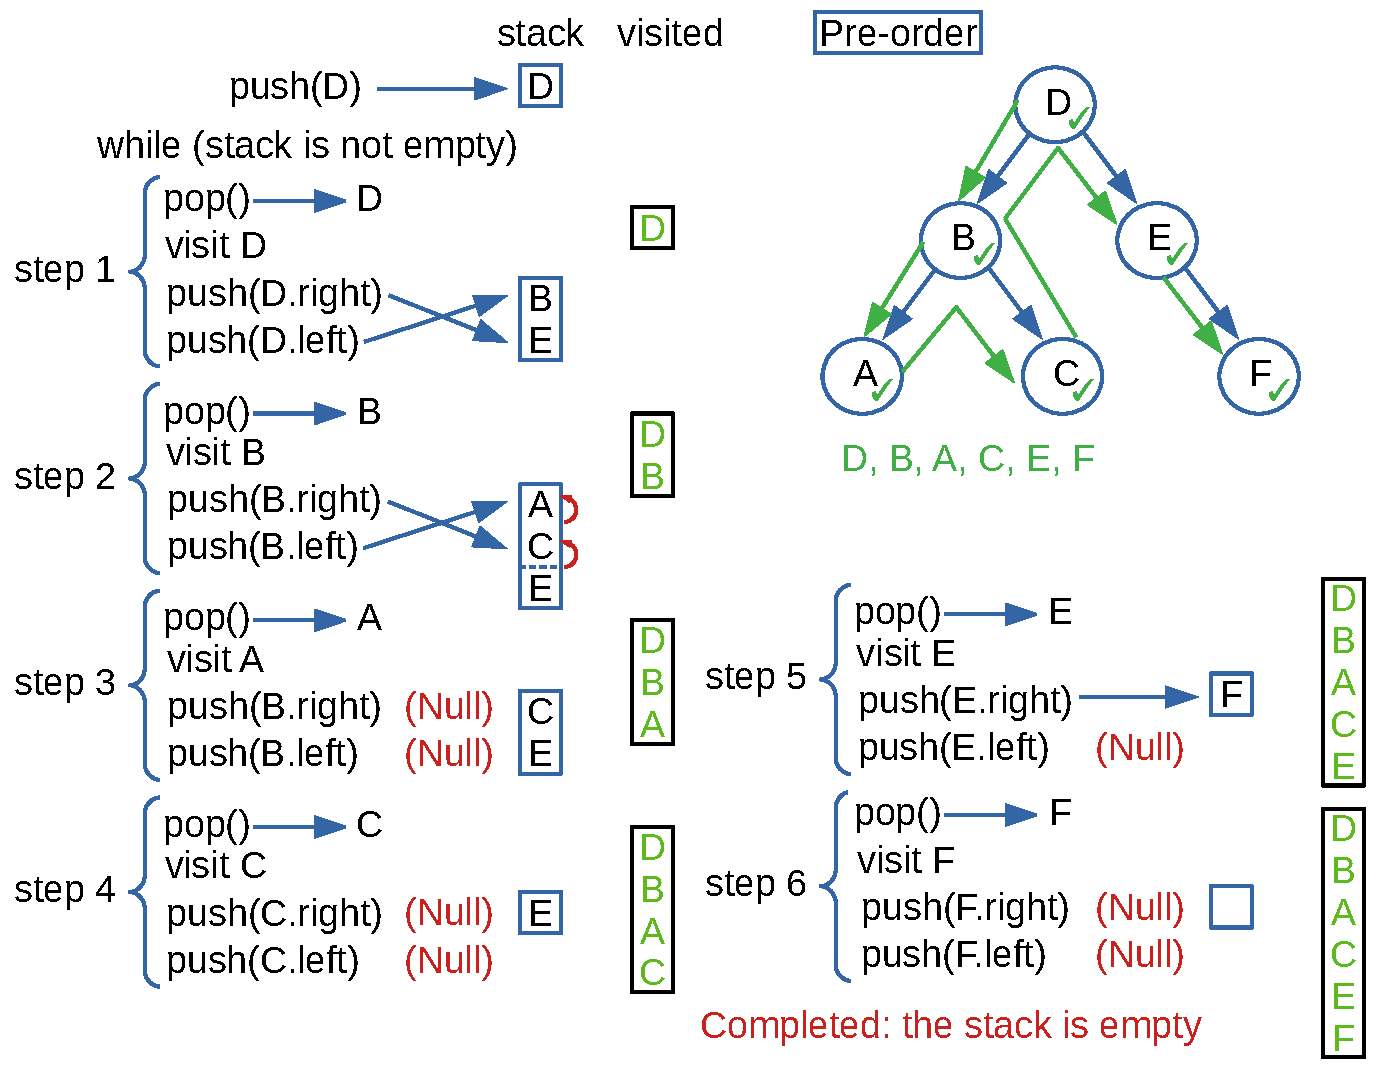
\includegraphics[scale=.6]{/home/omar/Documenti/AlgorithmsNotes/algorithms-notes/chapters/appendix/images/appendixtree/treesappendix_1.pdf}
		\caption[Pre-order iterative implementation example.]{Pre-order iterative implementation example.}
		\label{appendixtrees_1}
	\end{center}
\end{figure}

\section{In-order Traversal}
\label{inorderappendix}
\begin{figure}[H]
	\begin{center}
		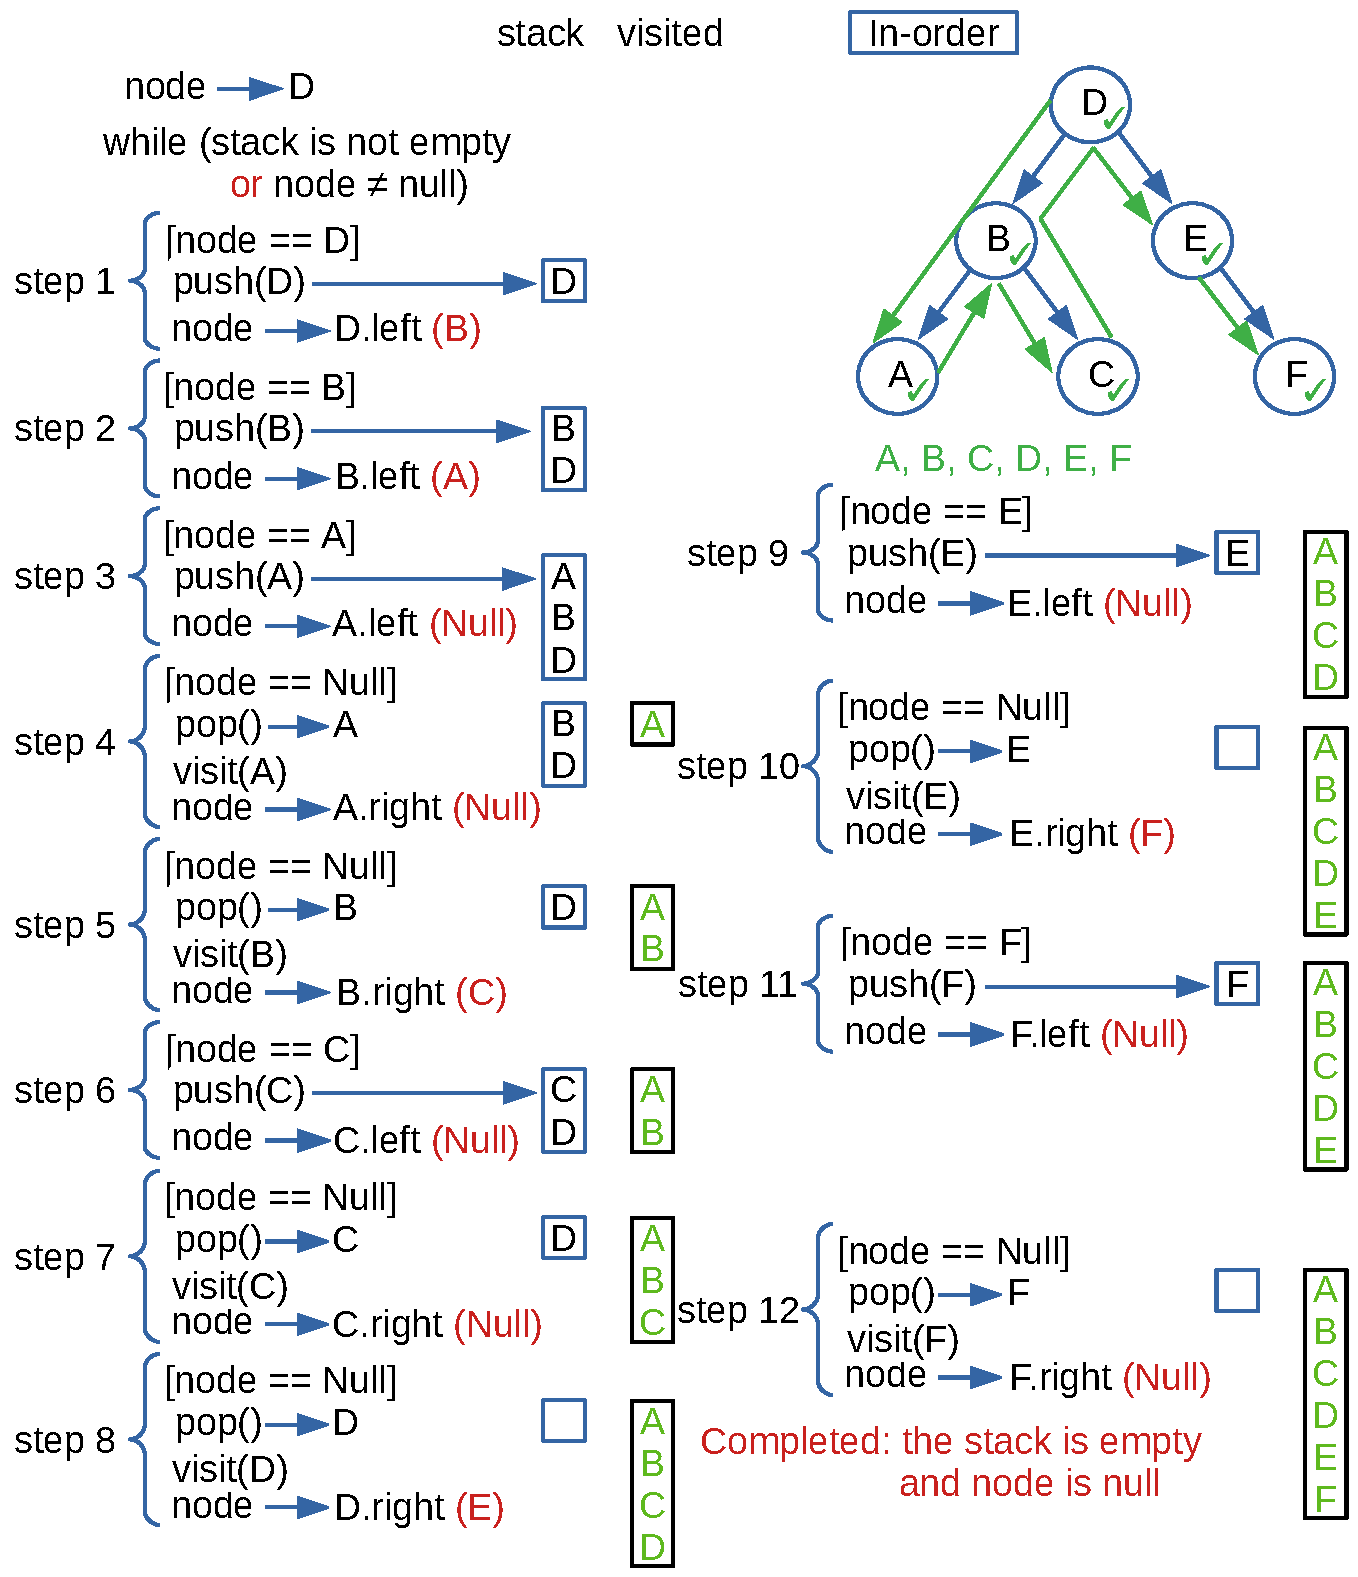
\includegraphics[scale=.6]{/home/omar/Documenti/AlgorithmsNotes/algorithms-notes/chapters/appendix/images/appendixtree/treesappendix_2.pdf}
		\caption[In-order iterative implementation example.]{In-order iterative implementation example.}
		\label{appendixtrees_2}
	\end{center}
\end{figure}

\begin{lstlisting}[firstnumber=1, caption={Tree operations implementation.}]
class BinaryTree():
	...

	def print_tree(self):
		return self.preorder_print(tree.root, "")[:-1]

	def preorder_search_recursive(self, start, find_val):
		if start:
			if start.value == find_val:
				return True
			else:
				return preorder_search_recursive(start.left, find_val) or
					   preorder_search_recursive(start.right, find_val)

	def preorder_search_iterative(self, start, find_val):
		if start == None:
			return None
		stack = []
		stack.push(start)
		while not stack: # Keep cycle until the stack is empty
			node = stack.pop()
			if node == find_val:
				return True
			# Right child is pushed first so that the left one is processed first
			if node.right:
				stack.push(node.right)
			if node.left:
				stack.push(node.right)

	def preorder_print(self, start, traversal):
		if start:
			traversal += (str(start.value) + "-")
			traversal = self.preorder_print(start.left, traversal)
			traversal = self.preorder_print(start.right,traversal)
		return traversal
\end{lstlisting}

\section{Post-order Traversal}
\label{postorderappendix}

\begin{lstlisting}[firstnumber=1, caption={Tree operations implementation.}]
class BinaryTree():
	...

	def print_tree(self):
		return self.preorder_print(tree.root, "")[:-1]

	def preorder_search_recursive(self, start, find_val):
		if start:
			if start.value == find_val:
				return True
			else:
				return preorder_search_recursive(start.left, find_val) or
					   preorder_search_recursive(start.right, find_val)

	def preorder_search_iterative(self, start, find_val):
		if start == None:
			return None
		stack = []
		stack.push(start)
		while not stack: # Keep cycle until the stack is empty
			node = stack.pop()
			if node == find_val:
				return True
			# Right child is pushed first so that the left one is processed first
			if node.right:
				stack.push(node.right)
			if node.left:
				stack.push(node.right)

	def preorder_print(self, start, traversal):
		if start:
			traversal += (str(start.value) + "-")
			traversal = self.preorder_print(start.left, traversal)
			traversal = self.preorder_print(start.right,traversal)
		return traversal
\end{lstlisting}

\begin{figure}[H]
	\begin{center}
		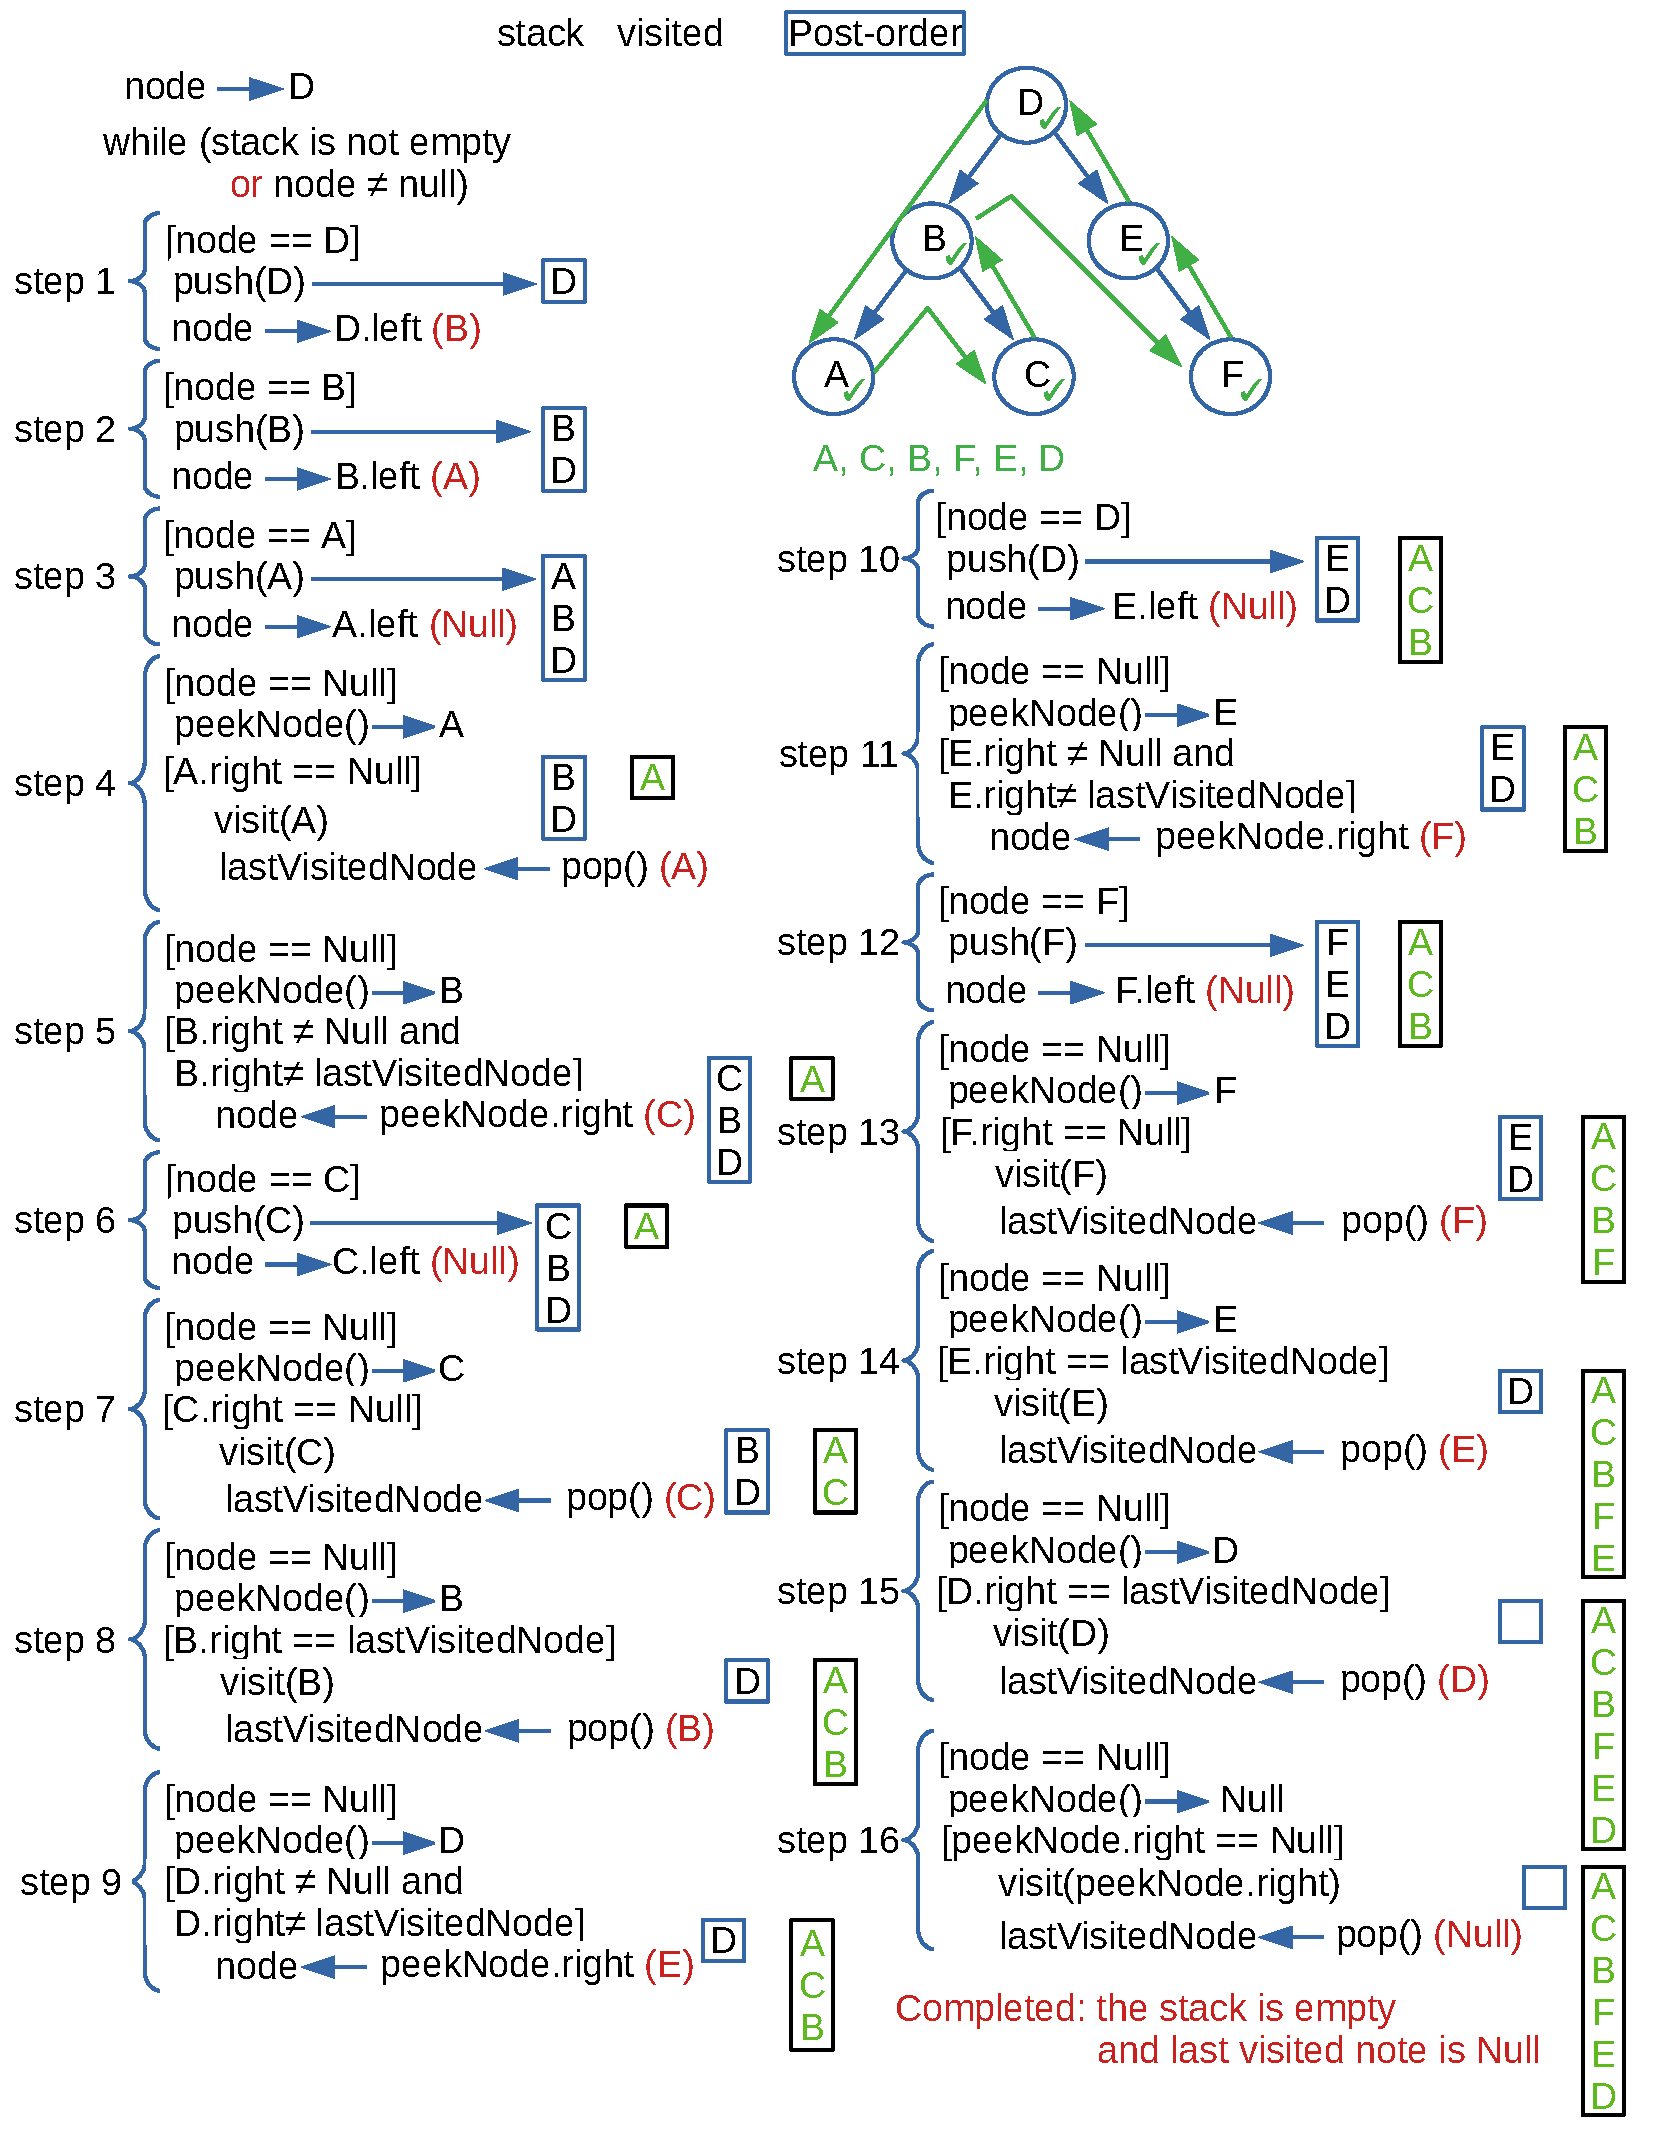
\includegraphics[scale=.6]{/home/omar/Documenti/AlgorithmsNotes/algorithms-notes/chapters/appendix/images/appendixtree/treesappendix_3.pdf}
		\caption[Post-order iterative implementation example.]{Post-order iterative implementation example.}
		\label{appendixtrees_3}
	\end{center}
\end{figure}

\section{Summary on Tree Traversal}
In the following figure (Figure \ref{appendixtrees_4}) there is a comprehensive schema of all different type of tree traversal in the depth-first search case.

\begin{figure}[H]
	\begin{center}
		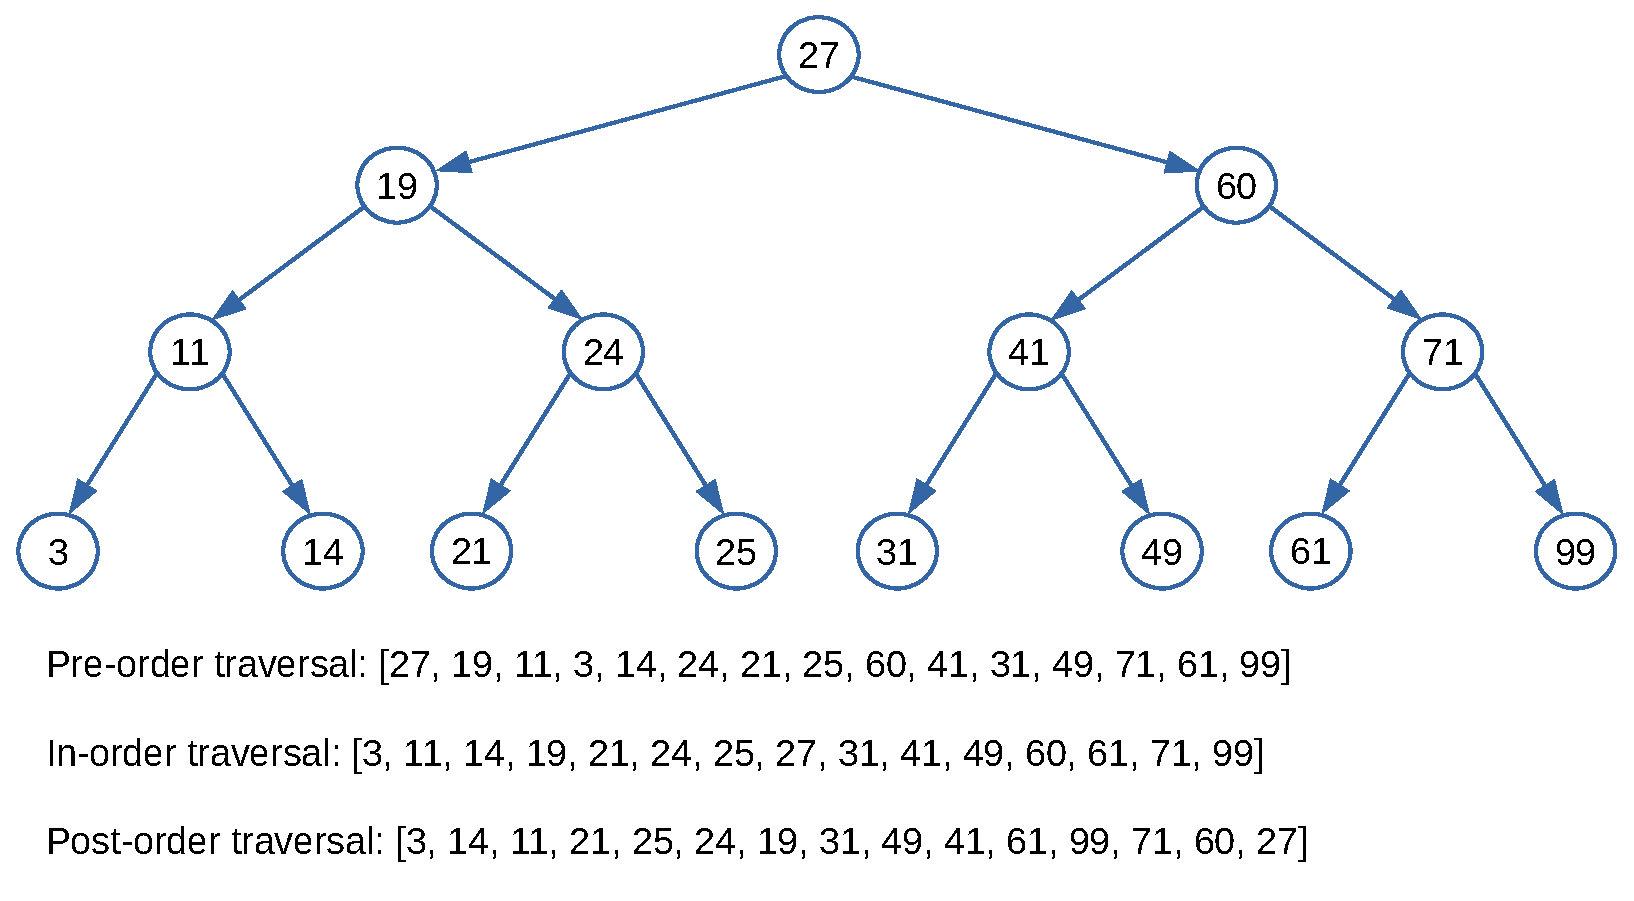
\includegraphics[scale=.6]{/home/omar/Documenti/AlgorithmsNotes/algorithms-notes/chapters/appendix/images/appendixtree/treesappendix_4.pdf}
		\caption[Example of all traversal type on a tree.]{Example of all traversal type on a tree.}
		\label{appendixtrees_4}
	\end{center}
\end{figure}